\documentclass[twocolumn,a4j]{jsarticle}
\setlength{\topmargin}{-20.4cm}
\setlength{\oddsidemargin}{-10.4mm}
\setlength{\evensidemargin}{-10.4mm}
\setlength{\textwidth}{18cm}
\setlength{\textheight}{26cm}

\usepackage[top=15truemm,bottom=25truemm,left=15truemm,right=15truemm]{geometry}
\usepackage[latin1]{inputenc}
\usepackage{amsmath}
\usepackage{amsfonts}
\usepackage{amssymb}
\usepackage[dvipdfmx]{graphicx}
\usepackage[dvipdfmx]{color}
\usepackage{listings}
\usepackage{listings,jvlisting}
\usepackage{geometry}
\usepackage{framed}
\usepackage{color}
\usepackage[dvipdfmx]{hyperref}
\usepackage{ascmac}
\usepackage{enumerate}
\usepackage{tabularx}
\usepackage{cancel}
\usepackage{scalefnt}

\renewcommand{\figurename}{Fig.}
\renewcommand{\tablename}{Table }

\lstset{
basicstyle={\ttfamily},
identifierstyle={\small},
commentstyle={\smallitshape},
keywordstyle={\small\bfseries},
ndkeywordstyle={\small},
stringstyle={\small\ttfamily},
frame={tb},
breaklines=true,
columns=[l]{fullflexible},
xrightmargin=0zw,
xleftmargin=3zw,
numberstyle={\scriptsize},
stepnumber=1,
numbersep=1zw,
lineskip=-0.5ex
}

\makeatletter
\def\@maketitle
{
\begin{center}
{\LARGE \@title \par}
\end{center}
\begin{flushright}
{\large 報告書 NO.07 - 3\quad\@date\quad\@author}
\end{flushright}
\par\vskip 1.5em
}
\makeatother

\setcounter{tocdepth}{3}

\author{来代 勝胤}
\title{令和3年度 11月 第3週 報告書}
\date{2021/11/25}

\begin{document}
\columnseprule=0.1mm

\maketitle
\section*{報告内容}
\begin{enumerate}[1.]
    \item 進捗状況
    \item 卒業研究について
    \item 実験について
    \item 研究計画
\end{enumerate}

\section{進捗状況}
今週は,卒業研究に向けた研究目的・方針・計画の検討を行った.
また,実施する実験について具体的な比較条件と
その形状の断面二次モーメントの算出を行い
現実的に可能な比較対象であるか検討した.

\section{卒業研究について}
\subsection{研究目的}
    $x$軸,$y$軸方向に取り付けられたひずみセンサについて,
    作用力の方向による出力電圧への影響・取付部の断面形状の違いによる影響を調べ,
    その関係から作用力実験結果の出力電圧を荷重に適切に変換する方法を模索し,提案する.
    \par
    また,その結果から選定された断面形状の取付部を高感度ひずみセンサを用いて作成し,
    現在使用しているひずみセンサとの比較実験を行うことで,その改善結果を示す.\\

\subsection{研究方針}
    \begin{enumerate}[(1)]
        \item 従来の実験装置について,作用力の方向による出力電圧の変化を調べる.
        \item [$\rightarrow$] 現在の実験装置の特徴を理解し,
              これまでの出力電圧から作用力への変換課程における問題点を明確にする.
        \item (1)の実験について,異なる幾つかの断面形状で実験を行い,
              出力電圧のひずみセンサ取付部の断面形状による違いを調べる.
        \item [$\rightarrow$] 断面形状の違いがどのような影響を及ぼすのかを明らかにし,
              2ゲージ法での測定の際に望ましい断面形状を提案する.
        \item (2)の結果より選定された断面形状の取付部を高感度ひずみセンサを用いて作成し,
              再度同様の実験を行う.
        \item [$\rightarrow$] 現在使用しているひずみセンサとの比較実験を行うことで,
              その改善結果を示す.
    \end{enumerate}
\newpage
\subsection{研究計画}
今後の研究計画について以下の表に示す.
11月・12月上旬にかけて実験装置を製作し,
12月中旬には実験を行う.
年始には結果を取り終えて1月下旬から卒業論文に本格的に着手する予定である.
\begin{figure}[htbp]
    \footnotesize
    \begin{center}
        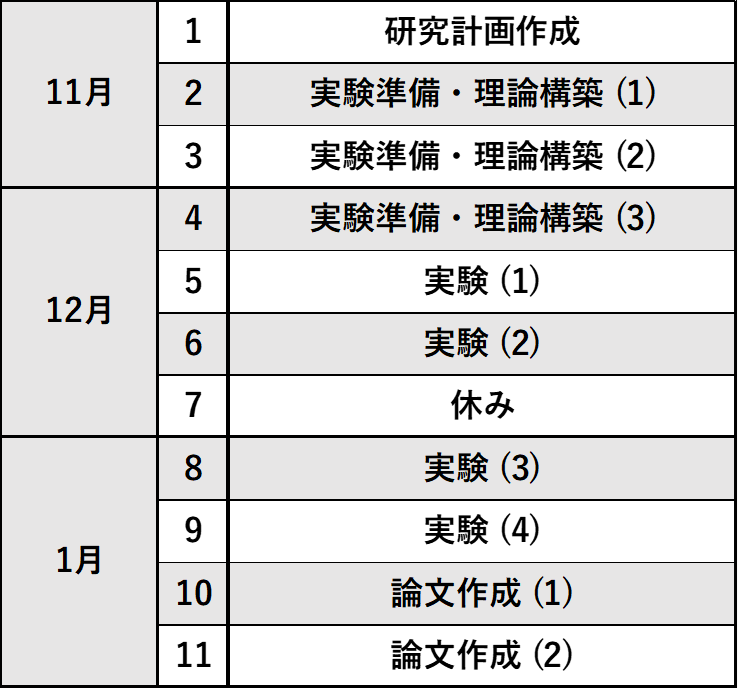
\includegraphics[width=70mm]{../images/monthly_plan.png}
        \caption{Research plan}
    \end{center}
\end{figure}
\section{実験について}
\subsection{実験条件}
以下の3種の断面形状について,比較実験を行う.
なお,現在の実験装置で使用されている (1)円筒を基準とし,
同等の断面二次モーメントを持つ形状とした.
\begin{enumerate}[(i)]
    \item 円筒  (外形:$D_1=\;$20.0[mm],内径:$D_2=\;$18.0[mm])
    \item 円   (直径:$D$)
    \item 正方形 (辺の長さ:$L$)
\end{enumerate}
\begin{figure}[htbp]
    \footnotesize
    \begin{center}
        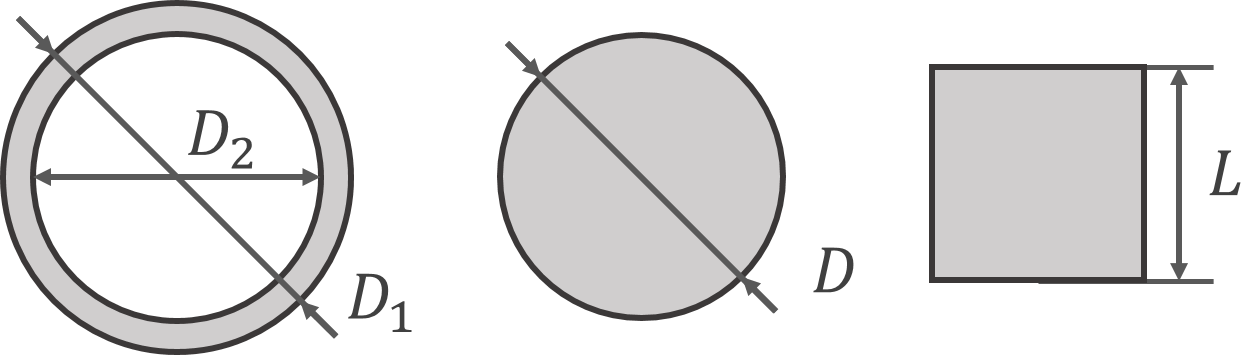
\includegraphics[width=80mm]{../images/testpieces_2.png}
        \caption{Cross-sectional shape of test pieces}
    \end{center}
\end{figure}
\newpage
\subsection{断面二次モーメントの算出}
(i)の円筒を基準に算出した断面二次モーメントを以下に示す.
なお、記号は上記の”実験条件”に対応している.
\begin{itembox}[l]{算出した形状の寸法}
    \begin{enumerate}[(i)]
        \item 円柱 $\cdots$ $D_1=\;$20.0 [mm],$D_2=\;$18.0 [mm]
        \item 円筒 $\cdots$ $D=\;$15.3 [mm]
        \item 角柱 $\cdots$ $L=\;$13.4 [mm]
    \end{enumerate}
\end{itembox}
\subsection{導出過程}
    \begin{itembox}[l]{円の断面二次モーメント}
        \begin{center}
            $\displaystyle I = \frac{\pi}{64}D^4\;\left(D:直径\right)$
        \end{center}
    \end{itembox}
    \begin{itembox}[l]{正方形の断面二次モーメント}
        \begin{center}
            $\displaystyle I = \frac{1}{12}L^4\;\left(L:辺の長さ\right)$
        \end{center}
    \end{itembox}
    \par
    \begin{enumerate}[(i)]
        \item 円筒 (外形:$D_1=\;$20.0[mm],内径:$D_2=\;$18.0[mm])
        \begin{eqnarray*}
            I &=& \frac{\pi}{64} \left(20^4 - 18^4\right)\\
            &=& \frac{\pi}{64} × 55024\\
            &=& 2700.98 \dots\\
            &\approx& 2701.0
        \end{eqnarray*}
        \item 円 (直径:$D$)
        \begin{eqnarray*}
            I &=& \frac{\pi}{64}D^4\\
            \frac{\pi}{64} × 55024 &=& \frac{\pi}{64}D^4\\
            \\
            D^4 &=& 55024\\
            \\
            D&=& 15.31\dots\\
            &\approx& 15.3 \left[\mathrm{mm}\right]
        \end{eqnarray*}
        \item 正方形 (辺の長さ:$L$)
        \begin{eqnarray*}
            I &=& \frac{1}{12}L^4\\
            2701.0 &=& \frac{1}{12}L^4\\
            \\
            L^4 &=& 2701.0 * 12\\
            &=& 32412\\
            \\
            L&=& 13.41\dots\\
            &\approx& 13.4 \left[\mathrm{mm}\right]
        \end{eqnarray*}
    \end{enumerate}
\end{document}